\documentclass{article}
\usepackage{amsmath}
\usepackage[utf8]{inputenc}
\usepackage{graphicx}
\usepackage{verbatim}
\usepackage{float}
\usepackage[makeroom]{cancel}
\usepackage[english]{babel}
\usepackage{textcomp}
\usepackage{gensymb}
\usepackage{color}
\usepackage{subcaption}
\usepackage{caption}
\usepackage{hyperref}
\usepackage{physics}
\usepackage{dsfont}
%\usepackage{amsfonts}
\usepackage{listings}
\usepackage{multicol}
\usepackage{units}

% From Eirik's .tex
\usepackage{epstopdf}
\usepackage{cite}
\usepackage{braket}
\usepackage{url}
\bibliographystyle{plain}

\usepackage{algorithmicx}
\usepackage{algorithm}% http://ctan.org/pkg/algorithms
\usepackage{algpseudocode}% http://ctan.org/pkg/algorithmicx

\usepackage[margin=1cm]{caption}
\usepackage[outer=1.2in,inner=1.2in]{geometry}
% For writing full-size pages
%\usepackage{geometry}
%\geometry{
%  left=5mm,
%  right=5mm,
%  top=5mm,
%  bottom=5mm,
%  heightrounded,
%}

% Finding overfull \hbox
\overfullrule=2cm

\lstset{language=IDL}
 %\lstset{alsolanguage=c++}
\lstset{basicstyle=\ttfamily\small}
 %\lstset{backgroundcolor=\color{white}}
\lstset{frame=single}
\lstset{stringstyle=\ttfamily}
\lstset{keywordstyle=\color{red}\bfseries}
\lstset{commentstyle=\itshape\color{blue}}
\lstset{showspaces=false}
\lstset{showstringspaces=false}
\lstset{showtabs=false}
\lstset{breaklines}
\lstset{aboveskip=20pt,belowskip=20pt}

\lstset{basicstyle=\footnotesize, basewidth=0.5em}
\lstdefinestyle{cl}{frame=none,basicstyle=\ttfamily\small}
\lstdefinestyle{pr}{frame=single,basicstyle=\ttfamily\small}
\lstdefinestyle{prt}{frame=none,basicstyle=\ttfamily\small}
% \lstinputlisting[language=Python]{filename}


\definecolor{codepurple}{rgb}{0.58,0,0.82}
\definecolor{backcolour}{rgb}{0.95,0.95,0.92}
\definecolor{dkgreen}{rgb}{0,0.6,0}
\definecolor{gray}{rgb}{0.5,0.5,0.5}
\definecolor{magenta}{rgb}{0.58,0,0.82}

\lstdefinestyle{pystyle}{
  language=Python,
  aboveskip=3mm,
  belowskip=3mm,
  columns=flexible,
  basicstyle={\small\ttfamily},
  backgroundcolor=\color{backcolour},
  commentstyle=\color{dkgreen},
  keywordstyle=\color{magenta},
  numberstyle=\tiny\color{gray},
  stringstyle=\color{codepurple},
  basicstyle=\footnotesize,
  breakatwhitespace=false,
  breaklines=true,
  captionpos=b,
  keepspaces=true,
  numbers=left,
  numbersep=5pt,
  showspaces=false,
  showstringspaces=false,
  showtabs=false,
  tabsize=2
}

%%%%%%%%%%%%%%%%%%%%%%%%%%%%%%%%
% Self made macros here yaaaaaay
\newcommand\answer[1]{\underline{\underline{#1}}}
\newcommand\pd[2]{\frac{\partial #1}{\partial #2}}
\newcommand\red[1]{\textcolor{red}{\textbf{#1}}}
\newcommand\numberthis{\addtocounter{equation}{1}\tag{\theequation}}
% Usage: \numberthis \label{name}
% Referencing: \eqref{name}

% Some matrices
\newcommand\smat[1]{\big(\begin{smallmatrix}#1\end{smallmatrix}\big)}
\newcommand\ppmat[1]{\begin{pmatrix}#1\end{pmatrix}}

%%%%%%%%%%%%%%%%%%%%%%%%%%%%%%%%%
% Eirik's self made macros
\newcommand{\s}{^{*}}
\newcommand{\V}[1]{\mathbf{#1}}
\newcommand{\husk}[1]{\color{red} #1 \color{black}}
\newcommand{\E}[1]{\cdot 10^{#1}}
\newcommand{\e}[1]{\ \text{#1}}
\newcommand{\tom}[1]{\big( #1 \big)}
\newcommand{\Tom}[1]{\Big( #1 \Big)}
\newcommand{\tomH}[1]{\big[ #1 \big] }
\newcommand{\TomH}[1]{\Big[ #1 \Big]}
\newcommand{\tomK}[1]{ \{ #1 \} }
\newcommand{\TomK}[1]{\Big\lbrace #1 \Big\rbrace}
\newcommand{\bigabs}[1]{\left| #1 \right|}

% Section labeling
\usepackage{titlesec}% http://ctan.org/pkg/titlesec
\renewcommand{\thesubsection}{\arabic{subsection}}

% Title/name/date
\title{FYS4150 - Project 5\\$N$-body simulation of an open galactic cluster}
\author{Simen Nyhus Bastnes \& Eirik Ramsli Hauge}
\date{9. December 2016}

\begin{document}
\maketitle
\begin{abstract}
\begin{figure}[H]
\centering

\includegraphics[scale=0.5]{totoro.jpg}
\end{figure}
\end{abstract}
\subsection{Introduction}
In this project we will attempt to develop code for simulating open galactic clusters. Taking inspiration from an article by M. Joyce and co-workers \red{cite}, we will build a simple model of an open galactic cluster. \red{redundancy ftw} An open cluster is an object consisting of a few thousand gravitationally bound stars, created from the collapse of a molecular cloud.\\\\
First, we look at some of the physics behind our model, making sure to find ideal units to fit our timescale. Running our model for $N = 100$ particles, we check the stability of our system, and find an ideal smoothing function for the gravitational force to remove some of the numerical instabilities. Having done that, we check how long the system takes to stabilize, conservation of energy, and checking the fraction of particles ejected from the system. Looking at only the bound particles, we can check if our results are consistent with the virial theorem.\\\\
Finally, we increase the number of particles while keeping the total mass constant, to see how the radial density looks like. This can then be compared to well known profiles such as the Navarro-Frenk-White profile.

\subsection{Theory}
\red{brief theory about open clusters here or in introduction?}
\subsubsection{N-body simulation}
Earlier this fall, we developed code that simulated the our Solar system.
\begin{align*}
  F = -\frac{G M_1, M_2}{r^2}\numberthis\label{eq:newton}
\end{align*}
% def metal():

\subsubsection{Spherical top-hat model}
In order to find units of time that fit the timescale, we will take a short detour into perturbation theory. While solving analytically can be difficult (or impossible) beyond linear perturbation theory, there exists an analytical solution for the so-called ``spherical top-hat'' model \red{cite}. In this model, the perturbation is a sphere of radius $R$, with a uniform density inside. It can be shown that this model has a parametrised solution
\begin{align*}
  R &= A(1-\cos\theta)\numberthis\label{eq:top-hat}\\
  t &= B(\theta-\sin\theta)\\
  &A^3 = GMB^2 
\end{align*}
From equation \eqref{eq:top-hat}, we 
Page 18ish in cosmo1.5 lecture notes\\
collapse time, spherical top hat model, virialization.
Sphere completely collapses at $\theta = 2\pi$ \red{add image maybe?}

\subsubsection{Particle ejection}

\subsubsection{Virial theorem}
For a bound gravitational system in equilibrium, the virial theorem says that
\begin{align*}
  2\langle K\rangle &= -\langle V\rangle \numberthis\label{eq:virial}
\end{align*}
where $\langle K\rangle$ is the time-average kinetic energy of the system, and $\langle V\rangle$ is the time-average potential energy. By the ergodic hypothesis, we can assume that an average over a large enough system should give the same result as the time average. \red{do like this, or just blatantly copy from project as i can't find any creative ways to rewrite that} 
\subsubsection{Radial density of particles}
simple expression \red{meow}
\begin{align*}
  n(r) = \frac{n_0}{\Big(1+(\frac{r}{r_0})^4\Big)} \numberthis\label{eq:radial_dist}
\end{align*}
Navarro-Frenk-White profile
\begin{align*}
  \rho(r) &= \frac{\rho_0}{\frac{r}{r_0}\Big(1+\frac{r}{r_0}\Big)^2}\numberthis\label{eq:NFW}
\end{align*}
\subsubsection{Numerical solving}
velocity verlet
\subsection{Experimental}
The programs used in this project can be found in the GitHub repository \cite{GitHub}, in the \texttt{/src/} folder. When running the program it takes 4 command line arguments: \texttt{N}, \texttt{t\_coll}, \texttt{dt} and \texttt{eps}. \texttt{N} is the number of stars in our cluster, \texttt{t\_coll} is our time unit, based on the collision time, \texttt{dt} is the time step and \texttt{eps} is the smoothing factor used in the force calculation. All data written to file by the main program are stored in \texttt{/benchmarks/} where most of the data analysis were done by python programs stored in \texttt{/python/} and the figures and gifs can be found in \texttt{/figures/}. \\ \\
The simulation starts by randomly positioning different stars inside a sphere with radius R = 20 light years. Each star will have an individual mass where the total mass is forced to be 1000 solar masses and an initial velocity set to be 0 in all directions. \\
Once all the positions and masses have been set, we can find the forces acting between them. While using velocity verlet to simulate the behaviour we can also find the individual kinetic and potential energy of each star as well as the total kinetic and potential energy of the system. 
\subsection{Results}
%%%%%%%%%%%%%%%%%%%%%%%%%%%%%
%%%         task b        %%%
%%%%%%%%%%%%%%%%%%%%%%%%%%%%%
A simulation of N = 100 stars over a time of 4 collision times with a time step of 0.001 and eps set to 0 gives us the animation found in \husk{REF!}. From this animation we can see that we don't reach an equilibrium. \husk{Is this correct?}
\\ \\
%%%%%%%%%%%%%%%%%%%%%%%%%%%%%
%%%         task c        %%%
%%%%%%%%%%%%%%%%%%%%%%%%%%%%%
Letting our program run for different number of particles we found the total energy, the fraction of particles with positive total energy and the kinetic energy of the escaped particles. These results are shown below in figure \ref{fig:noeps}.

\begin{figure}[H]
\centering
\begin{subfigure}{0.49\textwidth}
	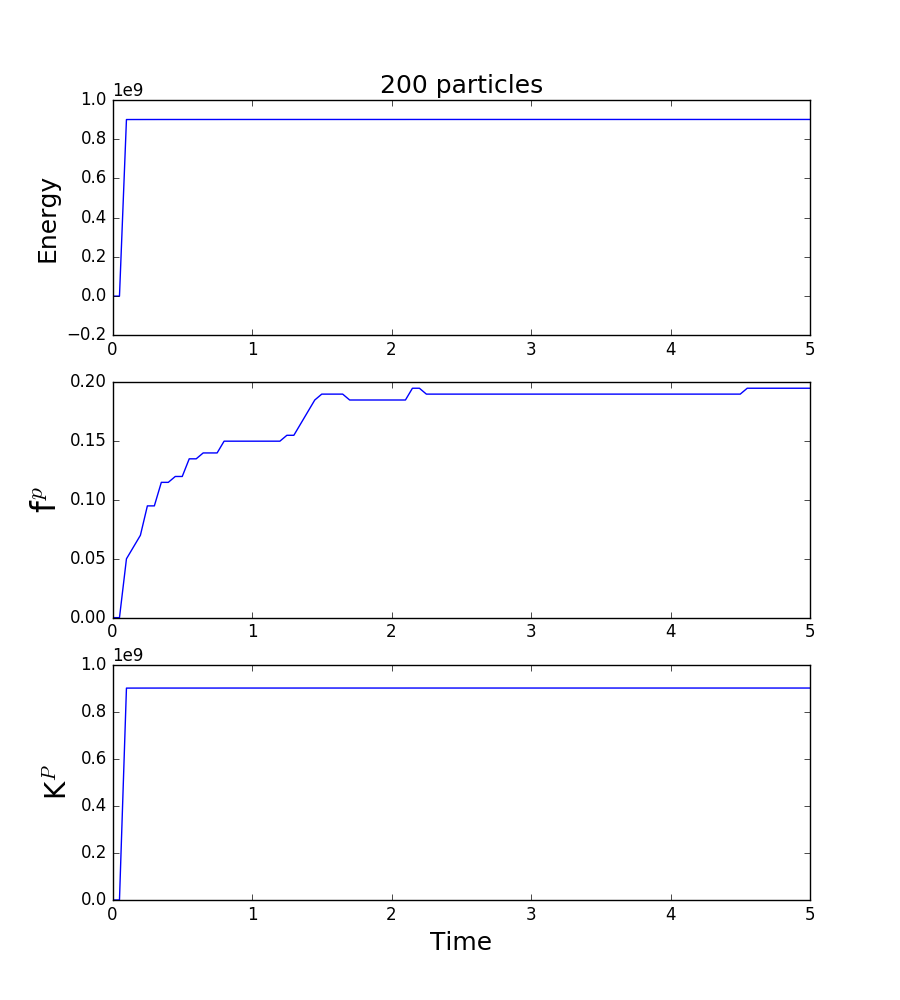
\includegraphics[scale=0.33]{{../figures/taskc/totenergy_N200}.png}
	\caption{Number of particles: 200}
	\label{subfig:noeps200}
\end{subfigure}
\qquad
\begin{subfigure}{0.49\textwidth}
	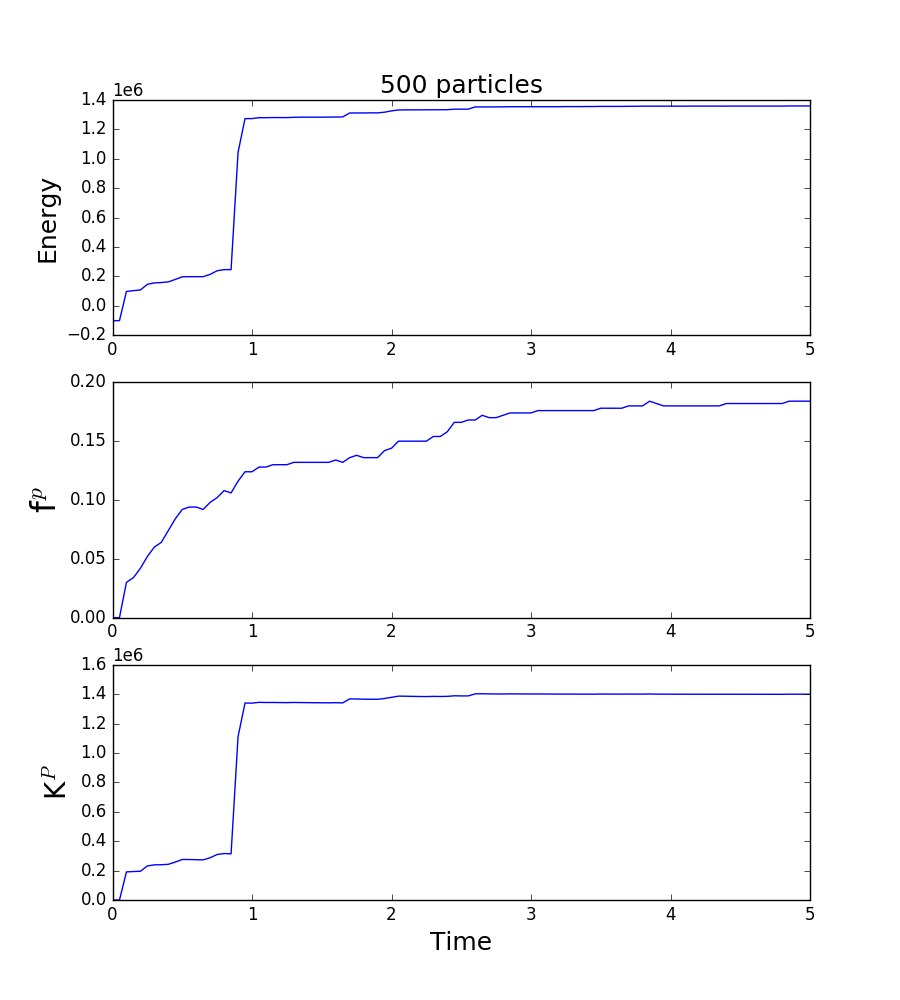
\includegraphics[scale=0.33]{{../figures/taskc/totenergy_N500}.png}
	\caption{Number of particles: 500}
	\label{subfig:noeps500}
\end{subfigure}
\begin{subfigure}{0.49\textwidth}
	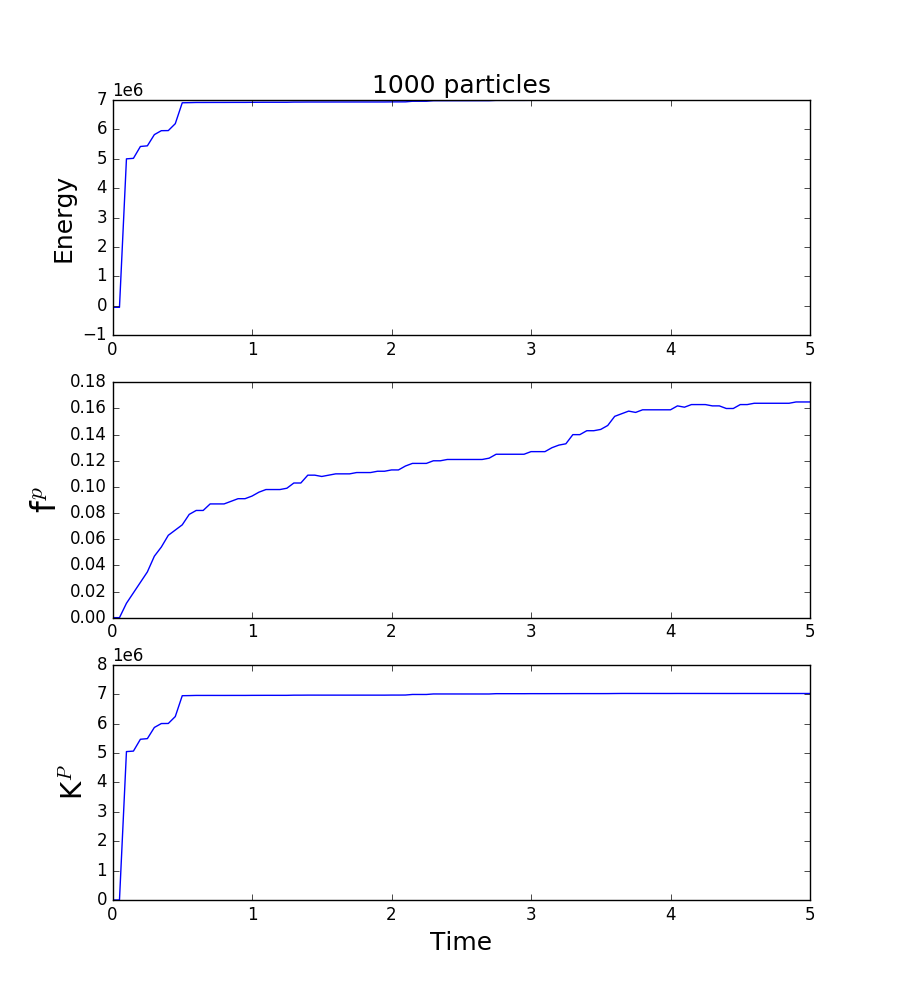
\includegraphics[scale=0.33]{{../figures/taskc/totenergy_N1000}.png}
	\caption{Number of particles: 1000}
	\label{subfig:noeps1000}
\end{subfigure}
\caption{Total energy and fraction of particles with positive total energy for different number of particles.}
\label{fig:noeps}
\end{figure}
%%%%%%%%%%%%%%%%%%%%%%%%%%%%%
%%%         task d        %%%
%%%%%%%%%%%%%%%%%%%%%%%%%%%%%
To find the best smoothing factor discussed above in the theory we used the trial and error method. For 200 stars with a time step of 0.001 and a time from 0 to 5 collision times we found the total energy as presented in figure \husk{fig:totalEnergy}
\begin{figure}[H]
\centering
\begin{subfigure}{0.49\textwidth}
	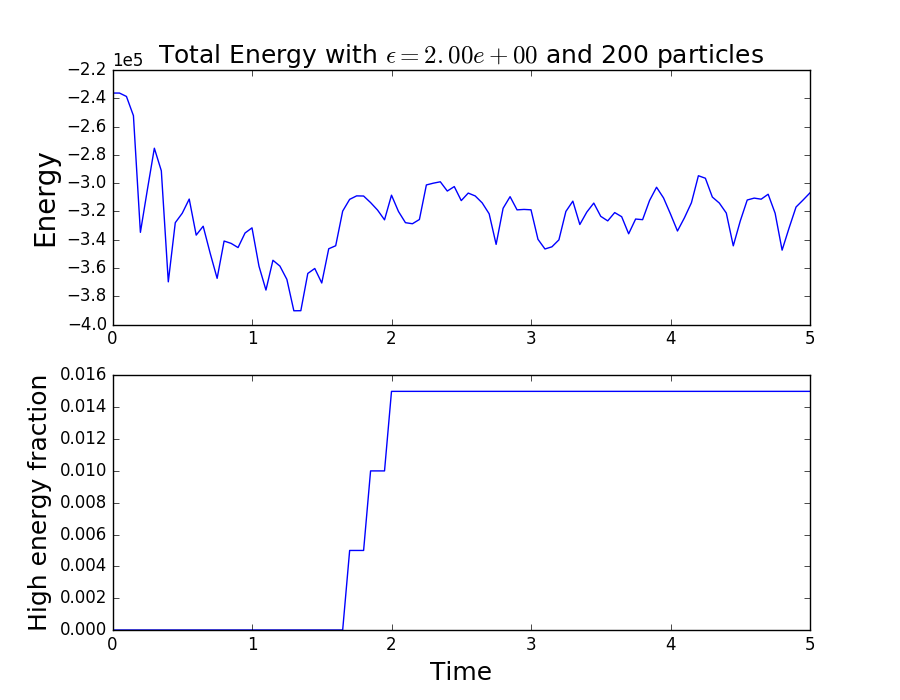
\includegraphics[scale=0.33]{{../figures/taskd/totenergy_eps2.00e+00_N200}.png}
	\caption{$\epsilon$ = 2.0}
	\label{subfig:eps2}
\end{subfigure}
\qquad
\begin{subfigure}{0.49\textwidth}
	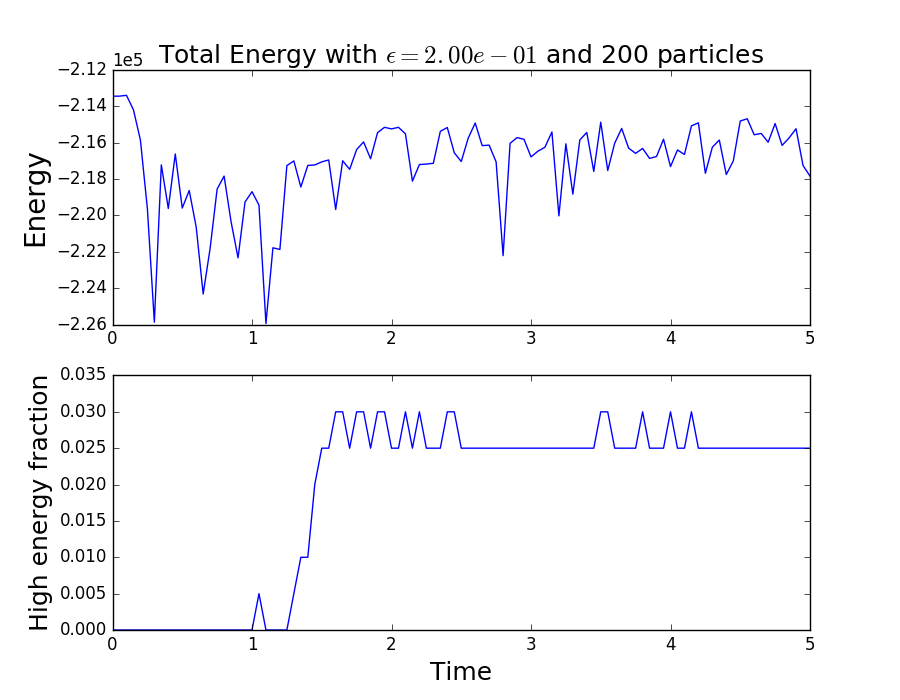
\includegraphics[scale=0.33]{{../figures/taskd/totenergy_eps2.00e-01_N200}.png}
	\caption{$\epsilon$ = 0.2}
	\label{subfig:eps0.2}
\end{subfigure}
\begin{subfigure}{0.49\textwidth}
	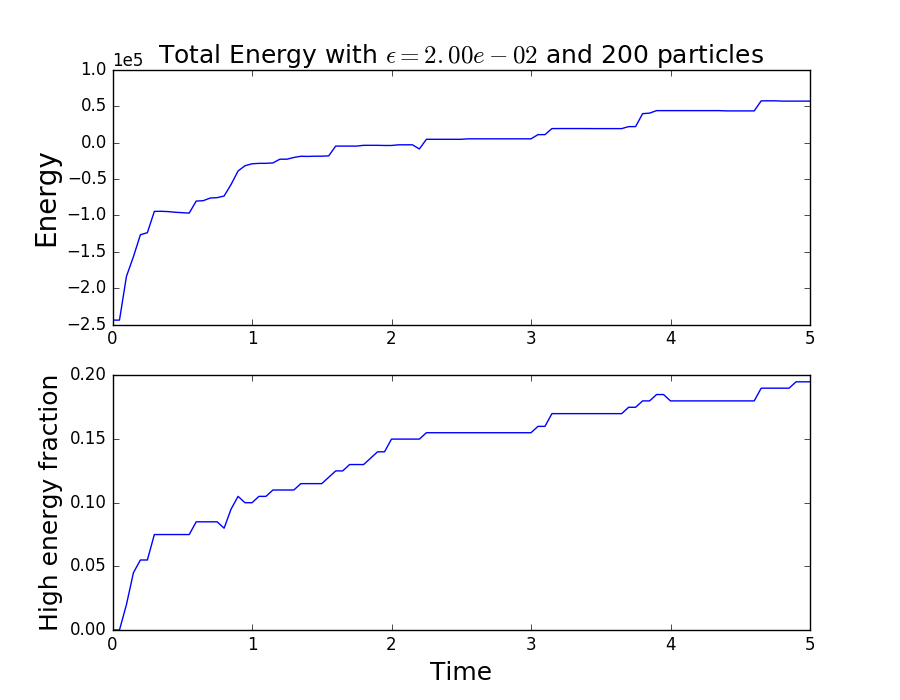
\includegraphics[scale=0.33]{{../figures/taskd/totenergy_eps2.00e-02_N200}.png}
	\caption{$\epsilon$ = 0.02}
	\label{subfig:eps0.02}
\end{subfigure}
\caption{Total energy and fraction of particles with positive total energy for different smoothing factors for a simulation of 200 stars.}
\label{fig:totalEnergy}
\end{figure}

%%%%%%%%%%%%%%%%%%%%%%%%%%%%%
%%%         task e        %%%
%%%%%%%%%%%%%%%%%%%%%%%%%%%%%
To see if we our results were consisten with the viral theorem, we checked if the average of the potential energy subtracted from two times the average of the bound particles kinetic energy  was zero. The result are plotted in figure \ref{fig:viral}
\begin{figure}[H]
\centering
\begin{subfigure}{0.49\textwidth}
	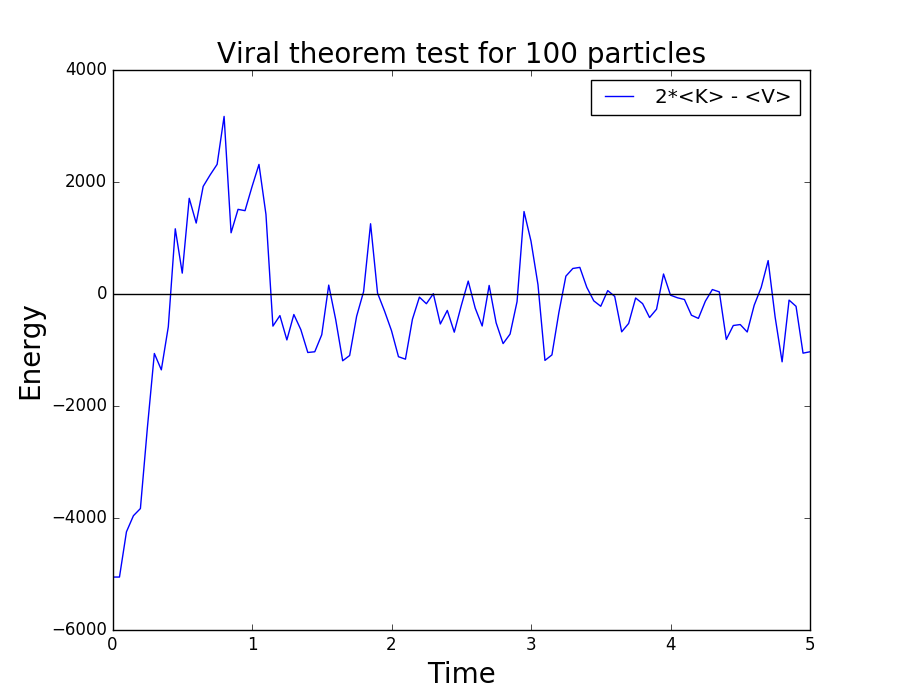
\includegraphics[scale=0.33]{{../figures/taske/viral_N100}.png}
	\caption{Number of particles: 100}
	\label{subfig:viral100}
\end{subfigure}
\qquad
\begin{subfigure}{0.49\textwidth}
	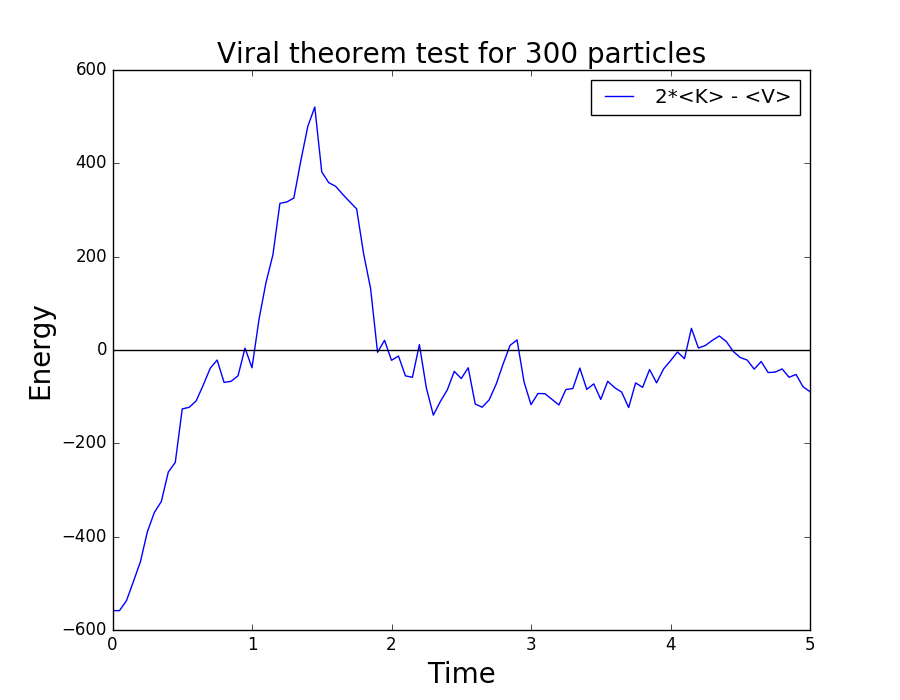
\includegraphics[scale=0.33]{{../figures/taske/viral_N300}.png}
	\caption{Number of particles: 300}
	\label{subfig:viral300}
\end{subfigure}
\begin{subfigure}{0.49\textwidth}
	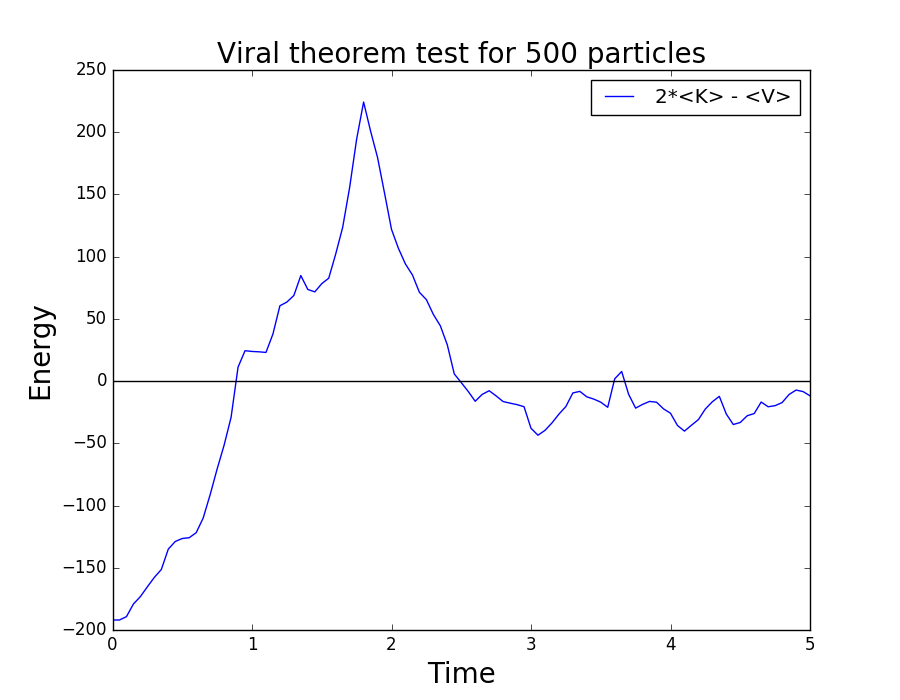
\includegraphics[scale=0.33]{{../figures/taske/viral_N500}.png}
	\caption{Number of particles: 500}
	\label{subfig:viral500}
\end{subfigure}
\caption{Total energy for different smoothing factors for a simulation of 200 stars.}
\label{fig:viral}
\end{figure}
%%%%%%%%%%%%%%%%%%%%%%%%%%%%%
%%%         task f        %%%
%%%%%%%%%%%%%%%%%%%%%%%%%%%%%
By simulating different number of particles with the same total mass we were able to find the radial density, mean distance from origo and the standard derivation of distance from origo (see figure \ref{fig:radialDens} and \ref{fig:meanstd})
\begin{figure}[H]
\centering
\begin{subfigure}{0.49\textwidth}
	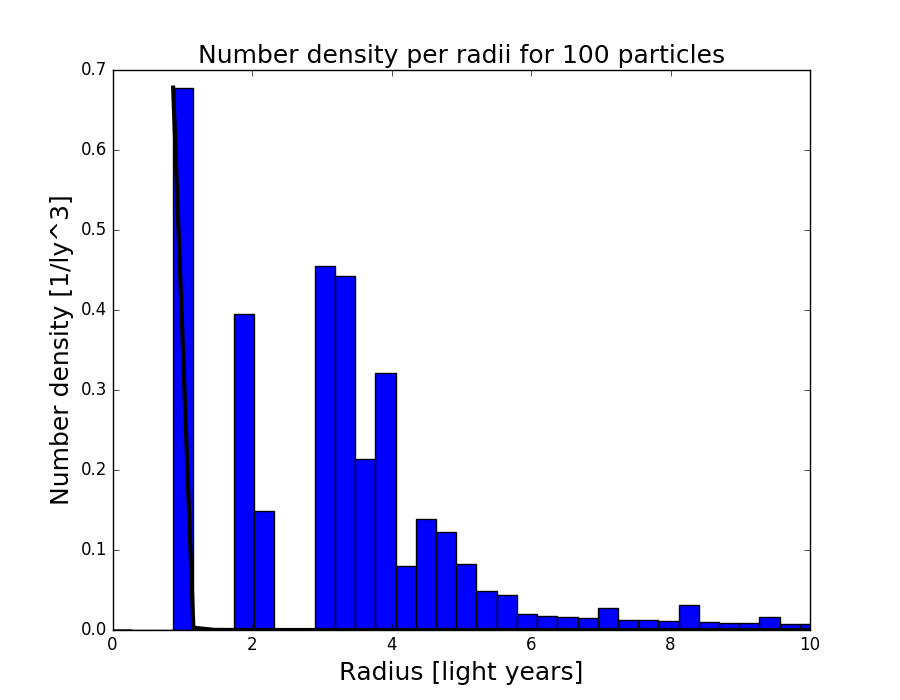
\includegraphics[scale=0.33]{{../figures/taskf/radialDens_N100}.png}
	\caption{Number of particles: 100}
	\label{subfig:radialDens100}
\end{subfigure}
\qquad
\begin{subfigure}{0.49\textwidth}
	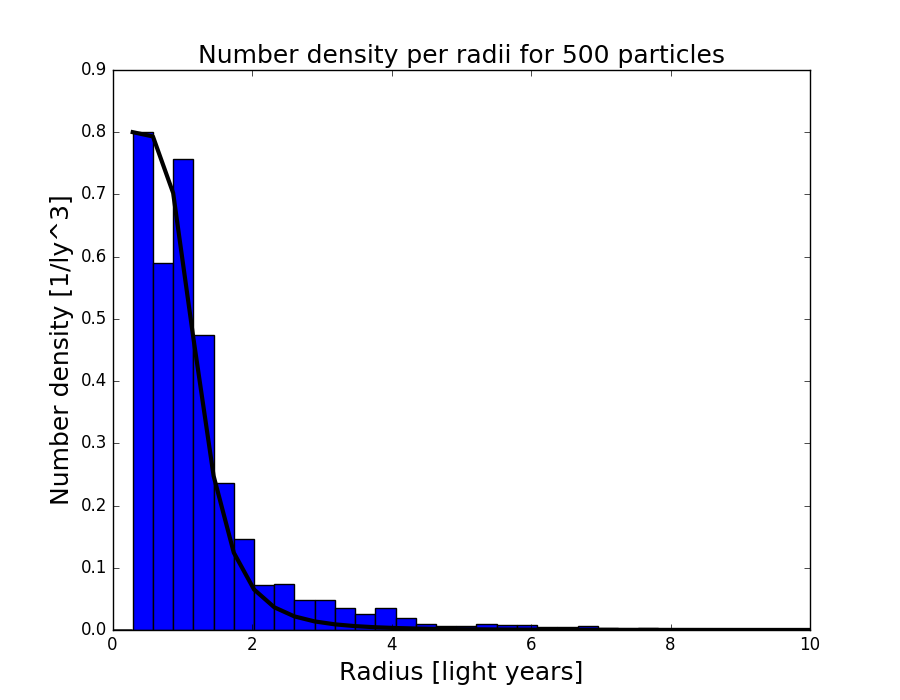
\includegraphics[scale=0.33]{{../figures/taskf/radialDens_N500}.png}
	\caption{Number of particles: 500}
	\label{subfig:radialDens500}
\end{subfigure}
\begin{subfigure}{0.49\textwidth}
	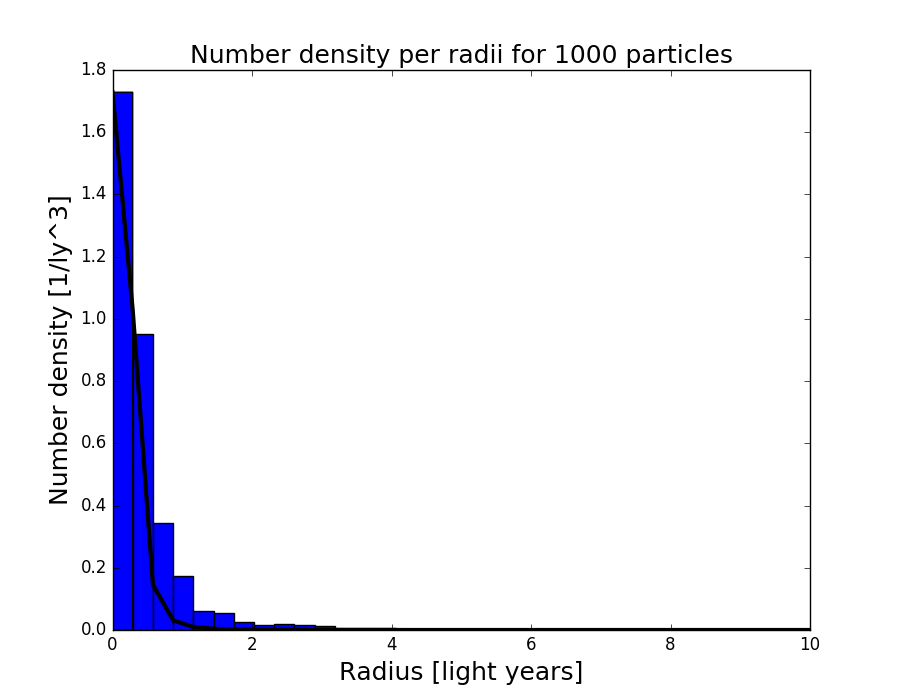
\includegraphics[scale=0.33]{{../figures/taskf/radialDens_N1000}.png}
	\caption{Number of particles: 1000}
	\label{subfig:radialDens1000}
\end{subfigure}
\caption{Radial density for different number of particles.}
\label{fig:radialDens}
\end{figure}
\begin{figure}[H]
\centering
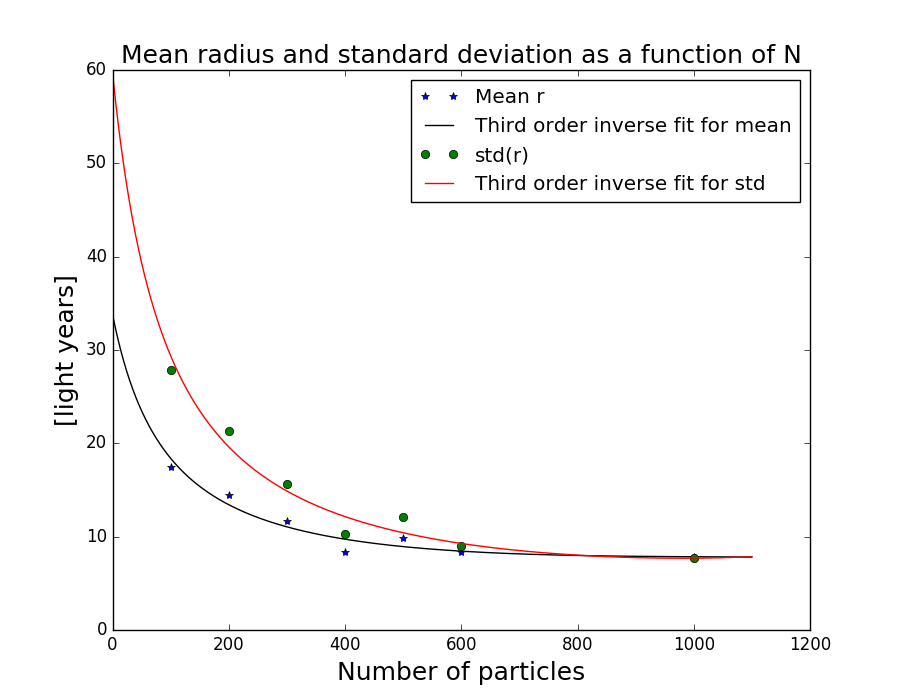
\includegraphics[scale=0.5]{{../figures/taskf/meanstd}.png}
\caption{Standard deviation and average distance from origo for all particles}
\label{fig:meanstd}
\end{figure}
\subsection{Discussion}
%%%%%%%%%%%%%%%%%%%%%%%%%%%%%
%%%         task a        %%%
%%%%%%%%%%%%%%%%%%%%%%%%%%%%%

%%%%%%%%%%%%%%%%%%%%%%%%%%%%%
%%%         task b        %%%
%%%%%%%%%%%%%%%%%%%%%%%%%%%%%

%%%%%%%%%%%%%%%%%%%%%%%%%%%%%
%%%         task c        %%%
%%%%%%%%%%%%%%%%%%%%%%%%%%%%%

%%%%%%%%%%%%%%%%%%%%%%%%%%%%%
%%%         task d        %%%
%%%%%%%%%%%%%%%%%%%%%%%%%%%%%

%%%%%%%%%%%%%%%%%%%%%%%%%%%%%
%%%         task e        %%%
%%%%%%%%%%%%%%%%%%%%%%%%%%%%%

%%%%%%%%%%%%%%%%%%%%%%%%%%%%%
%%%         task f        %%%
%%%%%%%%%%%%%%%%%%%%%%%%%%%%%
As we can see from figure \ref{fig:radialDens} the cluster is densest near origo. This is as expected 

\subsection{Conclusion}
\bibliography{references}
\end{document}
